\chapter{Non-obtrusive detection of emotions}
\label{ch:discussion}

The initial chapters of this thesis presented the theoretical foundations and the work needed to create a novel method for remote detection of emotions of users during the interaction with games. As highlighted by previous research, the understanding of human emotions, as well as the process of automatically detecting them, is the aim of several researchers in a many different fields. As detailed in Chapter \ref{ch:literature-games}, different theories have been proposed to model and study emotions in a variety of contexts, including those related to games. A considerable share of those theories is based on the human physiology, connecting emotional reactions to psychophysiological signals, e.g. HR and skin conductivity. Several approaches have been proposed to put such models and theories into practice to achieve the ultimate goal of detecting what a person is feeling. Chapters \ref{ch:literature-face} and \ref{ch:literature-physiological}, for instance, describe the connection between emotions and their manifestations in the body, particularly the process of mapping measurable psychophysiologicalsignals into an emotional state.

Emotion detection is a complex and multidisciplinary problem that demands knowledge from many different areas. In this thesis, focus has been given to the field of games research. Results and contributions of this research are aimed at and discussed under the light of games research, however they are likely to be useful for scholars in other fields as well. This chapter presents and discusses the outcomes of a research focused on creating a non-obtrusive method for emotion detection, particularly in the context of games. The following sections also present the insights obtained during the systematic investigation and development of the proposed method, including a discussion on how they relate to games research and other areas.

\section{Game-based model for emotion detection}

Commonly the process of detecting emotions using psychophysiological signals relies on mapping the patterns of such signals into an emotional state. As pointed by the literature review conducted in this thesis, a validated way of doing it is by measuring the changes of psychophysiological signals caused by the interaction with emotion elicitation materials. Generally the process involves three main parts: emotion elicitation, signal acquisition and the mapping of such signals into an emotional state. Simply put, subjects are exposed to materials that are accepted to produce certain emotional reactions, e.g. video and images depicting sad events, followed by observations of how the signals of interest, e.g. HR, change in accordance. Finally the emotion detection is performed by a technique aimed at producing a model to map the changes of those signals into emotional states, e.g. machine learning model like neural networks. The literature review presented in this thesis shows a myriad of different approaches used in each of the previously mentioned parts.

The majority of previous work focuses on producing a group model, where data from several individuals is used to created a trained machine able to detect emotions of any other subject outside the training population. Contrary to the established notion that a group model is better, this research investigated the venue of a user-tailored approach. As pointed by previous findings \parencite{something}, a model trained on data of a given person might be better at predicting the emotional state of such person. This is motivated by the fact that people are different in many aspects, including cultural and personal expectations \parencite{some}. Furthermore it is reasonable to believe that those individual characteristics might be preserved and better accounted for in a method that uses a user-tailored model as opposed to a group model to detect emotions. In this thesis, both the emotion elicitation process and the mapping of psychophysiological signals into emotional states were focused on the notion of the individual as opposed to the group.

\subsection{Calibration games as emotion elicitation}

%When games are used, they are usually gamified version of cognitive tests, or games featuring a well defined difficulty curve, e.g. easy/hard levels. Users have different gaming skills and expectations, so a game designed to be elicitate stresss might not be perceived as such by some users.

%, while previous work explored the use of games as elicitation sources for recognizing user emotions, relying on the emotional states a person can experience \citep{mandryk2006continuous} and which physiological signals are better predictors of such states \citep{jerritta2011physiological},

Previous works have used several different emotion elicitation materials, mainly images and videos, and less often game-focused elements. Those material, however, lack a more user-tailored approach for studying the variations of signals. Emotional states such as stress and boredom are often inducted by administering a game with the same particular setup, e.g. high/low difficulty, to all subjects. People respond differently to media according to their personality \cite{ravaja2004effects}, and they differ in social, learning and play styles \cite{goldberg1993structure}. A game session labeled as stressful, for instance, assumes that all subjects have the same expectations and behave similarly, which dilutes the individuality of each person as some might experience the interaction as not being stressful as intended. Additionally the analysis usually involves the interaction of subjects with some game levels (from the same game) featuring a constant difficulty scale, which does not contemplate the variations of signals in a context where the game difficulty is constantly increasing in the same game level/session.

Investigation of better game-based emotion elicitation materials was one of the main aspects of this research. Aiming to properly elicitate particular emotional states on each user, this research introduced the novel idea of calibration games. As detailed in Section \ref{sec:experiment1-games-elicitation} (on page \pageref{sec:experiment1-games-elicitation}), calibration games are carefully designed and developed games that have a difficulty level that constantly and linearly progresses over time without a pre-defined stopping point. At the beginning the games are highly predictive, without novelties, changes or surprises and with emphasis on the passage of time during a wait, which leads to an emotional state of boredom \cite{van2010behave,koster2013theory,schell2014art}. The game difficulty is then periodically increased until the subject is not able to cope with the challenges at hand, which happens at different times for different users. The ever-growing game difficulty leads to an emotional state of stress towards the end of the interaction, accounting for the expectations and gaming skill of a wide range of users.

Sections \ref{sec:experiment1-study1} and \ref{sec:experiment1-study2} presented a detailed analysis regarding how responses related to physiological activity, i.e. HR, and facial actions (FA), relate to emotional states in a game context featuring constant changes in difficulty (calibration games). Results show that the proposed idea of a calibration game is a valid emotion elicitation material which accounts for personal differences among subjects when inducing emotional states of stress and boredom. Using the proposed calibration games, it was possible to observe and confirm with statistical significance variations of HR and naked-eye recognizable FA that happened during the interactions with the games, especially under situations that were designed to provoke boredom and stress. Those findings were an essential part of the user-tailored method proposed in this thesis, since they proved that calibration games can be used as emotion elicitation material. Another important factor is the nature of the calibration games when compared to other emotional stimuli, e.g. images or videos. The use of images, videos or text as content to produce the emotional stimuli is less likely to produce the reactions of a real gaming session. In a game, users are in charge of actions, which are bound to have consequences. A bad judgment might cause the main character to get hurt, or a right movement might produce a reward. This feedback loop is happening constantly in a game, likely producing emotional reactions on the user. It is plausible to believe that the calibration games present a more sophisticated interaction through their game mechanics, as opposed to the simplistic, or even inexistent, interaction between users and images/videos, for instance. Consequentially the use idea and use of calibration games is likely to create a deeper emotional connection between users and the emotional elicitation material, resulting in clear and more observable changes in psychophysiological signals.

\subsection{Remote acquisition of psychophysiological signals}

This thesis focused on an emotion detection method whose elements used in each of the three previously mentioned parts are combined in a novel way, particularly in the field of games research. The majority of the novelty in the proposed approach relies on the use of calibration games as emotion elicitation, the remote acquisition of signals of interest and the use of a user-tailored approach to map that information into emotional states.

%however its reliability within a context involving natural behavior must be checked. The methods are sensitive to noise caused by movement, facial expressions or changes in illumination (e.g. screen activity reflected on user's face), which are all likely to happen in such sessions with natural behavior. Those interferences might produce unreliable measurements of the HR signal, resulting in misleading investigations. It is important to establish the reliability of remote HR measurements under situations with natural behavior, where users are not instructed to behave differently than what they usually do. In that light this paper presents an analysis of the remotely obtained HR signal of users within such natural context. We developed a set of casual-themed, similar to off-the-shelf games that were carefully designed to present stressful and boring moments, which should induce players to present variations of HR. During the gaming sessions, the player's HR signal was remotely estimated using the work by \textcite{poh2011advancements}, an established rPPG technique for HR estimation. A physical sensor was used as ground truth. A comparison and analysis of the accuracy of remote HR estimations are presented and discussed. The main contribution of this paper is the accuracy evaluation of an established rPPG technique within the context of gaming sessions where users behave naturally instead of following movement constraint rules, e.g. remain still. Our results provide researchers with information related to the reliability of a remote HR measurement technique when applied to contexts where users behave more naturally

%The use of remote measurement of physiological signals, such as rPPG, has already been applied to emotion detection. Signals as HR and HRV were used to remotely detect stress \parencite{mcduffcogcam, mcduff2014improvements, bousefsaf2013remote}, for instance. Since the estimations of rPPG techniques are significantly affected by external noise, e.g. subject's movement, experimental results are usually accompanied by accuracy evaluations regarding the estimations of the employed rPPG technique. In the majority of the cases, subjects are typically instructed to stay still \parencite{rouast2016remote}, which improves the accuracy of the rPPG technique. In some other cases, however, authors evaluate the accuracy of the HR estimation under scenarios where subjects are instructed to act naturally. Despite the fact that such works present experiments where subjects are told to behave naturally, their accuracy evaluation is based on artificial or simple human-computer interactions. Subjects are idly staring at the camera \parencite{zhao2013remote,hsu2014learning}, faking an interaction with a computer \parencite{poh2010non}, working on a task, i.e. make a website \parencite{monkaresi2014machine} or mentally subtract numbers \parencite{mcduff2014remote}, or performing arbitrary movements \parencite{tran2015robust}, e.g. head rotation in different degrees.


\section{Insights outside games research}

Here I will present some of the insights I gained during the whole process. I can mention how HR actually changes in the calibration games, hinting that researchers could use this information to create better models, for instance. I will also mention how the use of remote estimations of HR is a good tool, however it is extremely affected by natural movement (as detailed in study 3).

\section{Enhancing questionnaires in game research}

Here I will connect my research with its practical use. I will try to show how it can be used as a tool to enhance the use of questionnaires in game research. I could say that this approach can be used to replace questionnaires, but our numbers do not allow such a bold statement at the moment.


%\begin{figure}[h]
%    \centering
%    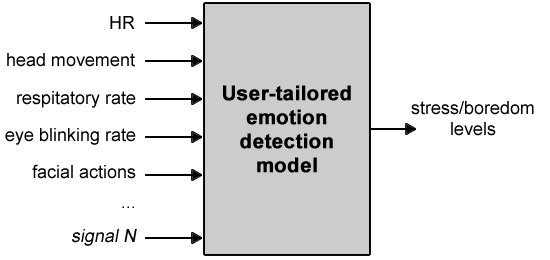
\includegraphics[width=0.6\textwidth]{figures/model-inputs-set.png}
%    \caption{Overall structure of the user-tailored emotion detection model regarding input (user signals) and output (stress/boredom levels).}
%    \label{fig:model-inputs-set}
%\end{figure}

%The user-tailored model proposed for this research might have $N$ input signals, varying from physiological ones, e.g. HR, to non-physiological ones, e.g. facial actions and head movements. Figure \ref{fig:model-inputs-set} illustrates the overall structure of the model. In order to be used in the model, an input signal needs to be supported by previous work regarding emotion detection, as well as be validated within the process of the proposed game-based calibration phase. Time and scope constraints limit the amount of input signals that can be implemented, evaluated and used in this research. As a consequence, a study will be conducted to investigate, validate and initially implement two of those signals into the proposed model: HR and facial activity (which includes head movement, lips activity, etc).

%The techniques and works presented in chapter \ref{ch:literature-face}, which relate to face detection and emotion estimation, suggest that facial analysis is an important component of a multifactorial emotion detection model. Empirical analysis of the data from the first experiment also suggest that individualities regarding facial activities do exist and could be used to estimate emotional states on a user-tailored basis \parencite{bevilacqua2016variations}. As described in section \ref{ch:literature-face-emotion-detection}, facial actions, head movement, lips/eye/mouth activity and distance measurements of detected facial landmarks are viable and proven sources of information for emotion detection.

%Regarding physiological signals, results indicate that the average HR mean for players during the last minute of gameplay is greater than the average HR mean during the second minute of gameplay (chapter \ref{ch:experiment1}, section \ref{s:study3}). The findings are aligned with and reinforce previous research that indicates higher HR mean during stressful situations in a gaming context. The findings also suggest that changes in the HR during gaming sessions is a promising indicator of stress.

%The study will involve the definition of how those two signals will be used as inputs for the model. Facial actions, for instance, will probably be detected and measured by the euclidian distance of the facial landmarks. A vector containing the distances will be evaluated as the input for the model. Regarding the HR, its mean and standard deviation during a particular analysis window will be evaluated as input for the model. A software for the detection of those two signals will be created and used to analyse the video recordings of the first experiment (chapter \ref{ch:experiment1}). The inclusion or exclusion of a component of a signal, e.g. variations of the distances of the lips landmark points, will be based on the accuracy to detect them and the frequency they appear in boring and stressful part of the calibration games.
